\documentclass[11pt]{article}

\usepackage[a4paper,margin=1in]{geometry}
\usepackage{amsmath,amssymb}
\usepackage{booktabs}
\usepackage{graphicx}
\usepackage{microtype}
\usepackage{siunitx}
\usepackage{url}
\usepackage[hidelinks]{hyperref}
\usepackage{enumitem}
\usepackage{caption}
\usepackage{subcaption}
\usepackage{xcolor}

\graphicspath{{figures/}}

\title{
    Beyond Closed-Set Recognition:
    Geometric Open-Set Detection for
    Kenyan Sign Language
}

\author{
    Rancy Chepchirchir
}

\date{}

\begin{document}

\maketitle

\begin{abstract}
Sign-language recognition systems are commonly evaluated
under closed-set assumptions in which every input is presumed
to belong to one of the classes observed during training.
This assumption is problematic for deployment because a model
may assign an unseen sign to a known vocabulary item with
substantial confidence rather than indicate that the input is
outside its learned vocabulary.

This work investigates this failure mode in a reconstructed
four-class Kenyan Sign Language (KSL) Transformer baseline
supporting the glosses \emph{father}, \emph{hello}, \emph{is},
and \emph{my}. We first reconstruct the checkpoint-compatible
landmark representation and extract 256-dimensional Transformer
embeddings. We then construct an embedding reference bank from
572 training samples and evaluate distance-based open-set
detection on 124 held-out in-distribution samples and 450
natural out-of-distribution videos drawn from 30 KSL glosses
outside the classifier vocabulary.

The closed-set classifier exhibits severe prediction collapse
on the expanded unseen-vocabulary set: 423 of 450 videos
(94.0\%) are assigned to the class \emph{my}, despite none
belonging to the supported vocabulary. In contrast,
nearest-neighbour distances in the learned embedding space
separate the held-out in-distribution and evaluated natural-OOD
samples. For mean 5-nearest-neighbour distance, the held-out
ID mean is 1.1207 and the natural-OOD mean is 12.9992.
The maximum observed held-out ID score is 7.4174, whereas
the minimum observed natural-OOD score is 10.1010, yielding
an empirical separation gap of 2.6836. Across
$k\in\{1,3,5,10,20\}$, the evaluated dataset yields AUROC
and AUPR of 1.0000 and FPR95 of 0.0000.

These results demonstrate a pronounced mismatch between
closed-set confidence and vocabulary membership in this
baseline, while showing that its learned representation
contains substantial information for detecting the evaluated
unseen KSL signs. The results should be interpreted as evidence
on the present model and datasets rather than as proof of
general open-set robustness.
\end{abstract}


\section{Introduction}

Automatic sign-language recognition has the potential to
improve accessibility to communication technologies, yet
recognition systems are frequently developed under a
closed-set classification assumption. Under this formulation,
a model receives an input sequence and must choose one label
from a predefined vocabulary. Such a system has no explicit
mechanism for stating that a valid sign lies outside its
training vocabulary.

This limitation is particularly important when a classifier
is deployed beyond the narrow conditions under which it was
trained. A sign-language video may contain an unseen lexical
item, a new signer, unusual landmark trajectories, incomplete
detections, or other forms of distribution shift. Standard
softmax classification nevertheless assigns probability mass
across the known classes. Consequently, a high predicted
probability need not imply that the input actually belongs
to the model's vocabulary.

In this work, we study this problem using a reconstructed
Kenyan Sign Language baseline. The underlying classifier
supports only four known glosses:
\emph{father}, \emph{hello}, \emph{is}, and \emph{my}.
Rather than treating the classifier output as an adequate
indicator of recognition reliability, we investigate the
geometry of its learned 256-dimensional representation.

Our central question is whether an embedding learned for
closed-set classification can also provide a useful signal
for open-set rejection. We therefore construct a reference
bank of training embeddings and score new inputs according
to their distance from nearby training representations.

The study makes four principal contributions:
\begin{enumerate}[leftmargin=*]
    \item We reconstruct and document the preprocessing path
    required to obtain checkpoint-compatible KSL landmark
    sequences and Transformer embeddings.

    \item We characterize the behaviour of the four-class
    classifier on natural KSL vocabulary outside its supported
    label set.

    \item We evaluate nearest-neighbour embedding distance as
    an open-set score using held-out known-class samples and
    450 natural unseen-vocabulary KSL videos spanning 30
    glosses.

    \item We expose the resulting open-set signal through the
    LughaLab inference API while retaining the original
    closed-set prediction for diagnostic transparency.
\end{enumerate}

The objective is not to claim that a simple distance detector
solves open-set KSL recognition generally. Instead, the
experiments ask a narrower and reproducible question:
\emph{does the representation learned by this particular
closed-set baseline contain sufficient geometric structure to
distinguish its known vocabulary from the evaluated natural
unseen vocabulary?}


\section{System and Representation}

\subsection{Landmark representation}

Each video is processed into a temporal sequence of landmark
features. The native extracted representation contains
225 floating-point features per detected frame. For
compatibility with the legacy checkpoint, the hand
coordinates occupy the first 126 dimensions and the remaining
99 dimensions are zero padded before application of the
checkpoint normalization statistics.

Let the extracted sequence be
\[
X =
\left[
x_1,\ldots,x_T
\right]^\top
\in
\mathbb{R}^{T\times225}.
\]

The checkpoint expects a sequence of length 64. Sequences
shorter than 64 frames are extended using repeat-last
padding, whereas longer sequences are uniformly temporally
downsampled. The resulting checkpoint-compatible sequence is

\[
\widetilde{X}
\in
\mathbb{R}^{64\times225}.
\]

Checkpoint-specific feature-wise standardization is then
applied using stored mean and standard-deviation statistics.

This representation was established through checkpoint
reconstruction experiments. It should therefore be understood
as a compatibility reconstruction and not as a claim that the
unpublished original training preprocessing has been recovered
exactly.


\subsection{Transformer embedding}

The reconstructed Transformer maps the normalized temporal
sequence to a 256-dimensional sequence-level representation.
We denote this mapping by

\[
z = f_{\theta}(\widetilde{X}),
\qquad
z\in\mathbb{R}^{256},
\]

where $f_{\theta}$ denotes the checkpointed encoder and $z$
is its sequence representation.

The classifier subsequently maps $z$ to four logits

\[
\ell = Wz+b,
\]

followed by the standard softmax transformation

\[
p(y=c\mid X)
=
\frac{
    \exp(\ell_c)
}{
    \sum_{j=1}^{4}\exp(\ell_j)
}.
\]

Because the softmax operates only over the four supported
classes, it cannot by itself express membership in an
unseen class.

\begin{figure}[t]
    \centering
    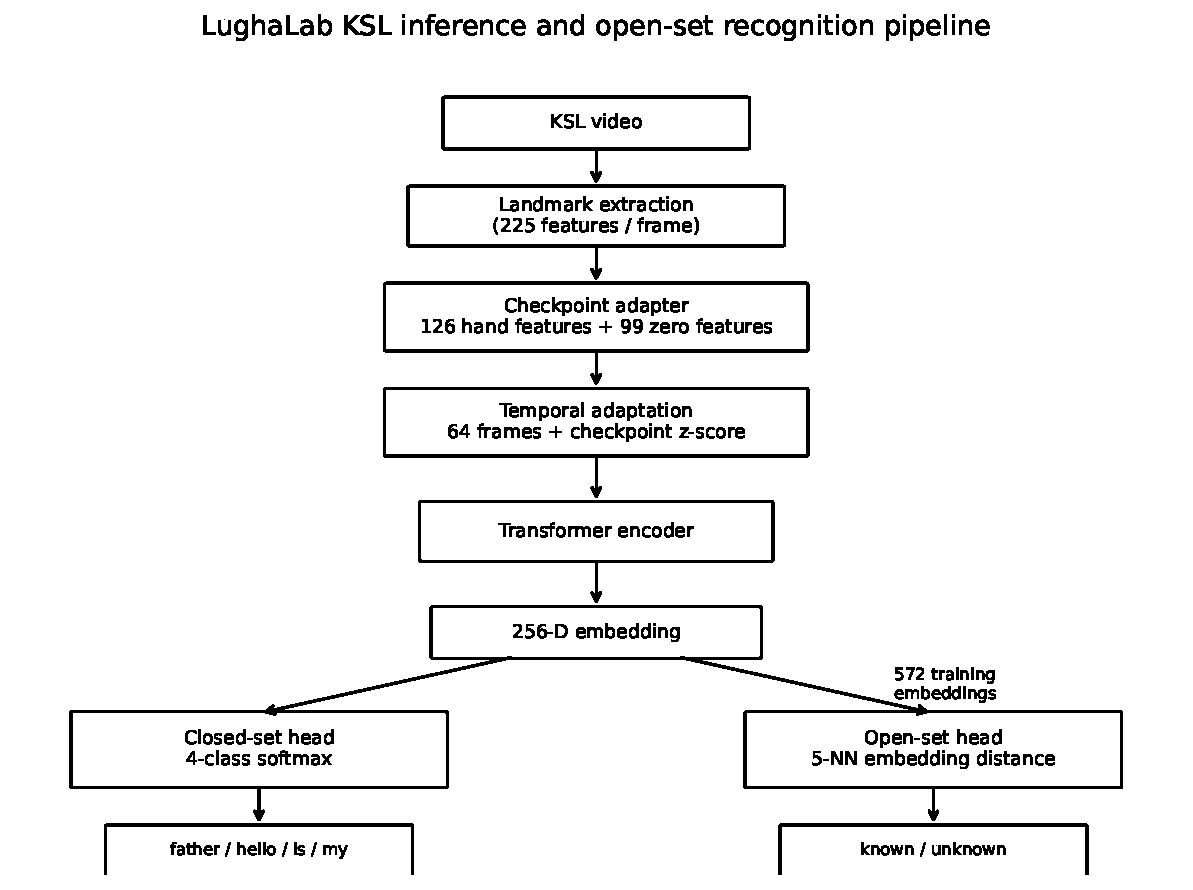
\includegraphics[
        width=\linewidth
    ]{fig01_open_set_architecture.pdf}
    \caption{
        LughaLab KSL inference architecture. Video landmarks
        are converted into the reconstructed checkpoint
        representation and encoded as a 256-dimensional
        sequence embedding. The original closed-set branch
        produces a four-class prediction, while the proposed
        open-set branch measures distance to the training
        embedding reference bank and can reject an input as
        unknown.
    }
    \label{fig:architecture}
\end{figure}


\section{Open-Set Detection}

\subsection{Embedding reference bank}

A reference bank is constructed from 572 training samples:

\[
\mathcal{B}
=
\left\{
(z_i,y_i)
\right\}_{i=1}^{572}.
\]

For a query embedding $z$, Euclidean distances to all
reference embeddings are computed:

\[
d_i(z)
=
\lVert z-z_i\rVert_2.
\]

Let
$d_{(1)}(z),\ldots,d_{(k)}(z)$
denote the $k$ smallest distances. The open-set score is
defined as the mean $k$-nearest-neighbour distance,

\[
S_k(z)
=
\frac{1}{k}
\sum_{j=1}^{k}
d_{(j)}(z).
\]

Larger values indicate that the query lies farther from
the training representation bank and is therefore more
geometrically novel.


\subsection{Decision rule}

Given threshold $\tau$, the open-set decision is

\[
\widehat{o}(z)
=
\begin{cases}
\mathrm{unknown},
&
S_k(z) > \tau,
\\[4pt]
\mathrm{known},
&
S_k(z) \leq \tau.
\end{cases}
\]

The runtime implementation uses $k=5$ and a provisional
threshold of

\[
\tau_{0.99}=5.4896,
\]

obtained from the 99th percentile of the held-out
in-distribution 5-NN score distribution.

The threshold is intentionally described as provisional:
it represents an empirical operating point for the current
baseline rather than a universally calibrated KSL
open-set threshold.


\section{Experimental Design}

\subsection{Known-class data}

The embedding reference bank contains 572 training examples
from the four supported classes. A separate held-out set of
124 known-class examples is used to characterize
in-distribution distance behaviour.

The held-out samples are not added to the reference bank.
This distinction is important because the open-set detector
must be evaluated against known-class examples that were not
used as reference points.


\subsection{Natural unseen-vocabulary data}

Natural OOD evaluation uses the eKitabu Kenyan Sign Language
video dataset. The dataset contains 2,237 videos spanning
30 gloss categories. Its provided split metadata contains
1,487 training, 300 validation, and 450 test videos.

For the expanded natural-OOD experiment, all 450 videos from
the provided test split are processed. There are 15 test
videos per gloss and 30 evaluated glosses. None of these
30 gloss labels belongs to the four-class vocabulary of the
baseline classifier.

All 450 videos were processed successfully. The mean landmark
detection rate was 0.8091, with a minimum of 0.1955.
The resulting natural-OOD embedding matrix has shape

\[
450\times256.
\]


\subsection{Evaluation metrics}

We evaluate $k$-NN distance detectors for

\[
k\in\{1,3,5,10,20\}.
\]

Reported measures include area under the receiver-operating
characteristic curve (AUROC), area under the
precision--recall curve (AUPR), false-positive rate at
95\% true-positive rate (FPR95), empirical score
distributions, and threshold-specific ID acceptance and OOD
rejection rates.

We additionally examine the relationship between geometric
novelty, maximum softmax probability, and landmark detection
coverage.


\section{Results}

\subsection{Closed-set behaviour on unseen vocabulary}

The most immediate result is that the four-class classifier
does not behave conservatively when presented with unseen
KSL vocabulary. Of the 450 natural-OOD videos, 423 are
classified as \emph{my}, 25 as \emph{hello}, and 2 as
\emph{is}. No video is assigned to \emph{father}.

Thus,

\[
\frac{423}{450}
=
0.9400
\]

of the entire unseen-vocabulary set collapses to a single
known class.

The average maximum softmax probability is 0.6916, with
values ranging from 0.3427 to 0.8348. Consequently,
substantial closed-set confidence occurs even though every
video in this experiment belongs to a gloss outside the
supported vocabulary.

\begin{figure}[t]
    \centering
    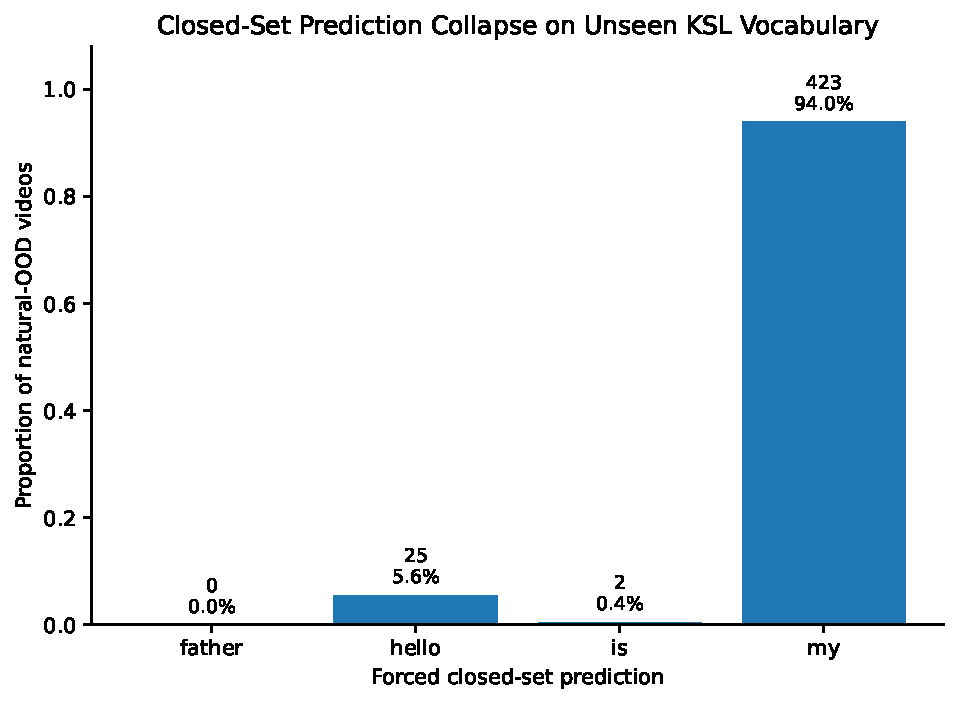
\includegraphics[
        width=0.78\linewidth
    ]{fig06_closed_set_collapse.pdf}
    \caption{
        Forced closed-set predictions for 450 natural KSL
        videos whose glosses are absent from the four-class
        classifier vocabulary. The model assigns 94.0\% of
        these videos to \emph{my}.
    }
    \label{fig:collapse}
\end{figure}


\subsection{Embedding-space separation}

The embedding-distance results differ sharply from the
closed-set softmax behaviour.

For the 5-NN detector, held-out ID samples have mean score

\[
\overline{S}_{5,\mathrm{ID}}
=
1.1207,
\]

whereas natural-OOD samples have mean score

\[
\overline{S}_{5,\mathrm{OOD}}
=
12.9992.
\]

The largest observed held-out ID score is 7.4174 and the
smallest natural-OOD score is 10.1010. Hence the evaluated
samples exhibit an empirical gap of

\[
10.1010 - 7.4174
=
2.6836.
\]

\begin{figure}[t]
    \centering
    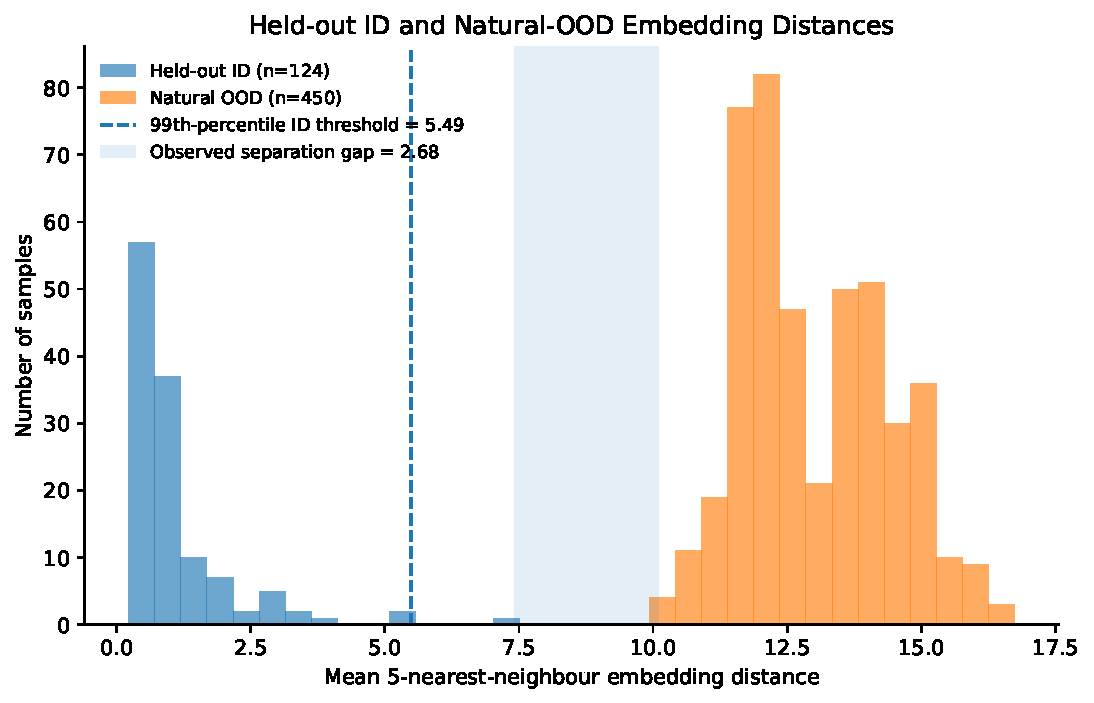
\includegraphics[
        width=0.82\linewidth
    ]{fig02_ood_score_distribution.pdf}
    \caption{
        Distribution of mean 5-nearest-neighbour embedding
        distances for held-out known-class data and expanded
        natural unseen-vocabulary KSL data. The shaded region
        marks the observed separation between the largest
        held-out ID score and smallest natural-OOD score.
    }
    \label{fig:distribution}
\end{figure}


\subsection{Neighbourhood-size sensitivity}

Table~\ref{tab:knn} reports performance for different values
of $k$. All evaluated neighbourhood sizes produce complete
ranking separation on the current dataset.

\begin{table}[t]
\centering
\caption{
Open-set detection performance across neighbourhood sizes.
Values describe the present held-out ID and natural-OOD
evaluation sets.
}
\label{tab:knn}
\begin{tabular}{
    r
    S[table-format=1.4]
    S[table-format=1.4]
    S[table-format=1.4]
    S[table-format=2.4]
    S[table-format=2.4]
}
\toprule
{$k$}
&
{AUROC}
&
{AUPR}
&
{FPR95}
&
{ID mean}
&
{OOD mean}
\\
\midrule
1  & 1.0000 & 1.0000 & 0.0000 & 0.8382 & 11.6127 \\
3  & 1.0000 & 1.0000 & 0.0000 & 0.9996 & 12.5170 \\
5  & 1.0000 & 1.0000 & 0.0000 & 1.1207 & 12.9992 \\
10 & 1.0000 & 1.0000 & 0.0000 & 1.3858 & 13.7757 \\
20 & 1.0000 & 1.0000 & 0.0000 & 1.7720 & 14.7601 \\
\bottomrule
\end{tabular}
\end{table}

\begin{figure}[t]
    \centering
    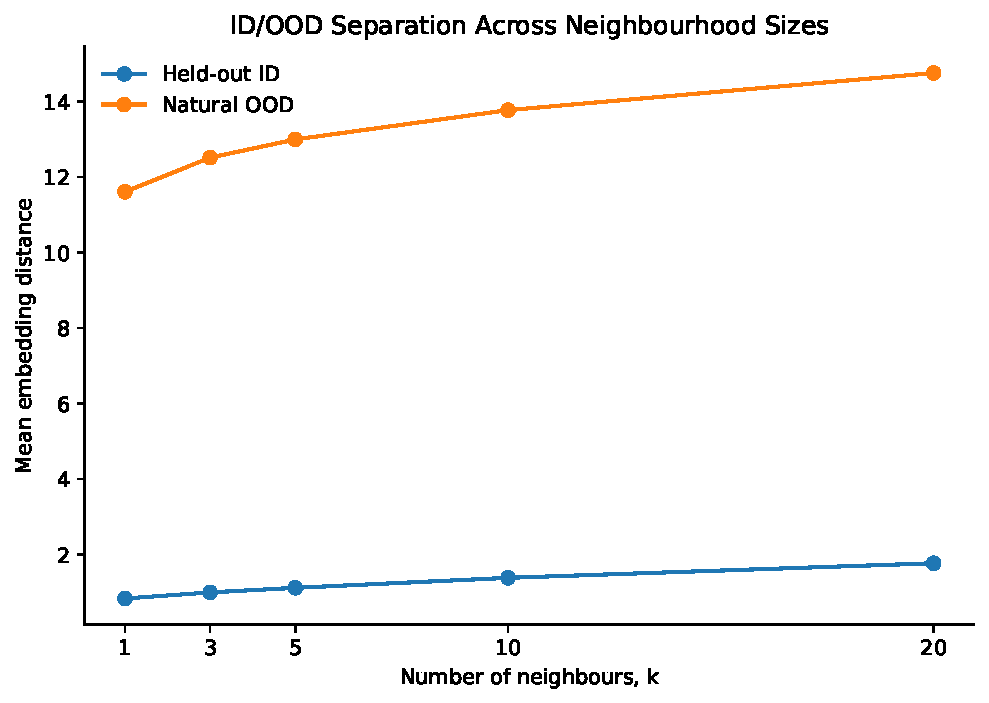
\includegraphics[
        width=0.76\linewidth
    ]{fig07_knn_comparison.pdf}
    \caption{
        Mean ID and natural-OOD embedding distances as the
        number of neighbours is varied.
    }
    \label{fig:k}
\end{figure}


\subsection{Threshold operating points}

For $k=5$, thresholds derived from held-out ID quantiles
produce the operating characteristics shown in
Table~\ref{tab:thresholds}.

\begin{table}[t]
\centering
\caption{
Empirical 5-NN operating points obtained from held-out
ID quantiles.
}
\label{tab:thresholds}
\begin{tabular}{
    S[table-format=2.1]
    S[table-format=1.4]
    S[table-format=1.4]
    S[table-format=1.4]
    S[table-format=1.4]
}
\toprule
{ID quantile (\%)}
&
{Threshold}
&
{ID accept}
&
{ID reject}
&
{OOD reject}
\\
\midrule
90.0 & 2.3673 & 0.8952 & 0.1048 & 1.0000 \\
95.0 & 3.1067 & 0.9435 & 0.0565 & 1.0000 \\
97.5 & 3.8914 & 0.9677 & 0.0323 & 1.0000 \\
99.0 & 5.4896 & 0.9839 & 0.0161 & 1.0000 \\
\bottomrule
\end{tabular}
\end{table}

At the provisional 99th-percentile threshold, 98.39\% of
the held-out ID examples are accepted and all 450 evaluated
natural-OOD examples are rejected.


\subsection{Variation across unseen glosses}

The separation is not produced by only a small number of
particularly distant unseen categories. At the 99th-percentile
threshold, every evaluated gloss has an OOD rejection rate
of 1.0000.

Mean 5-NN scores vary across glosses. For example,
\emph{agreement} has a mean score of 11.8429,
\emph{teach} 12.1715, \emph{market} 14.1230, and
\emph{ugali} 13.7618. Even the smallest individual
natural-OOD score in the expanded experiment, 10.1010,
remains above the largest observed held-out ID score.

\begin{figure}[t]
    \centering
    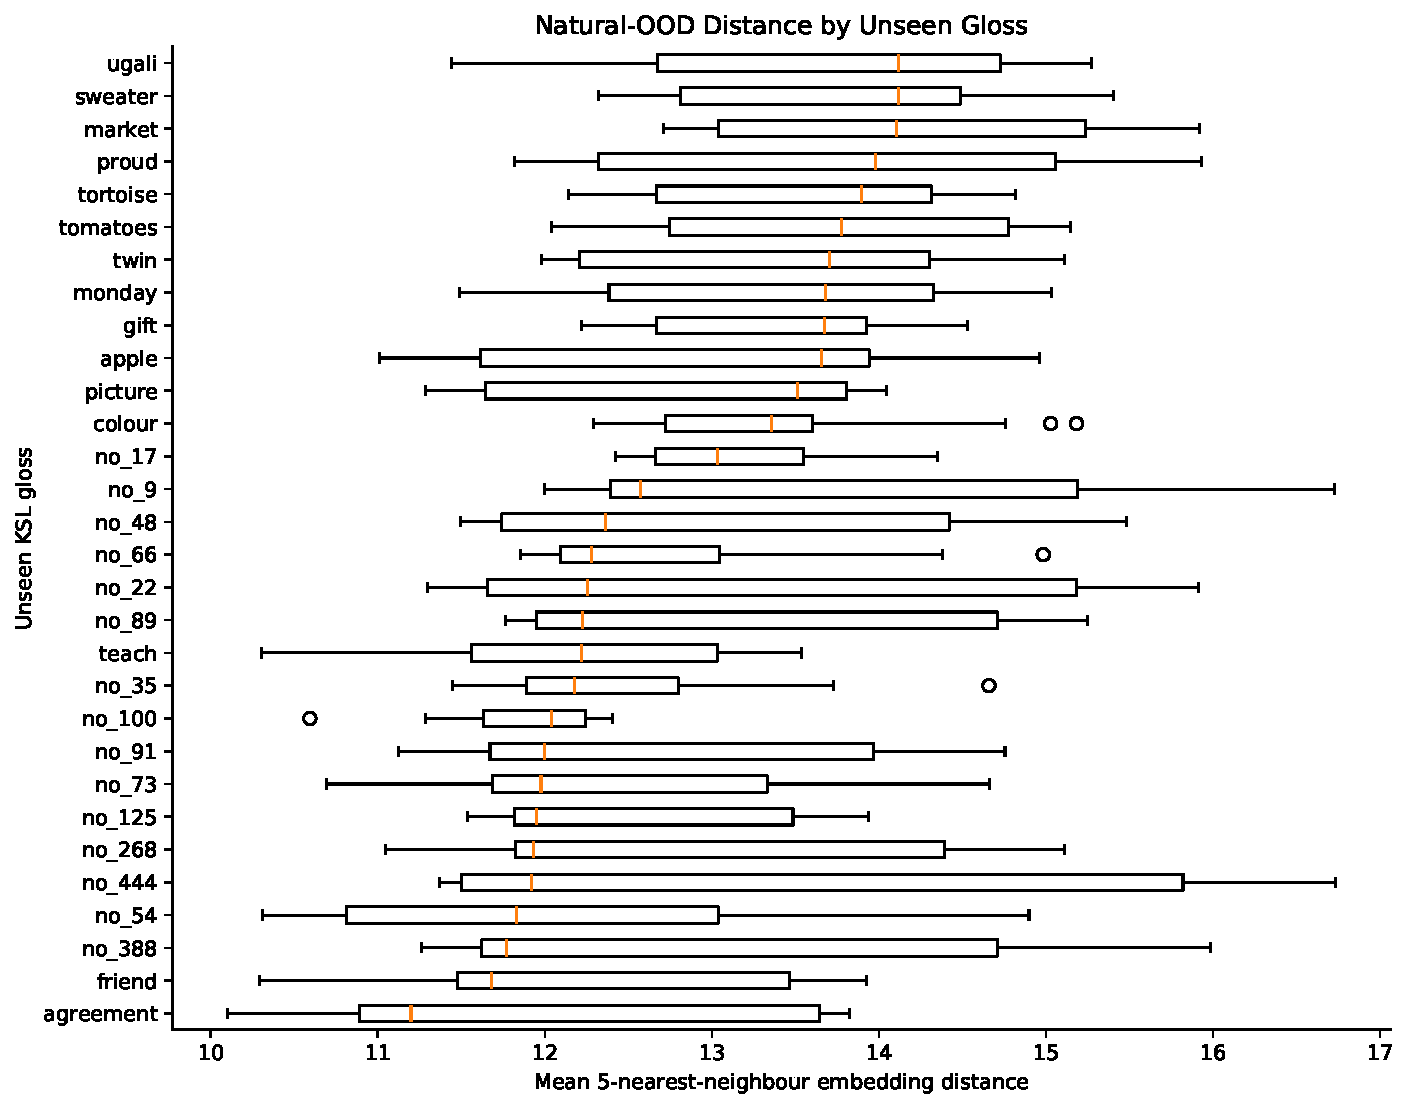
\includegraphics[
        width=0.92\linewidth
    ]{fig03_per_gloss_distance.pdf}
    \caption{
        Distribution of 5-NN embedding novelty scores across
        the 30 unseen KSL glosses in the expanded natural-OOD
        evaluation.
    }
    \label{fig:gloss}
\end{figure}


\subsection{Softmax confidence and geometric novelty}

Maximum softmax probability is negatively correlated with
the 5-NN novelty score:

\[
r=-0.6346.
\]

The relationship demonstrates that the classifier can become
less confident as inputs move farther from the training
representation, but this does not make softmax confidence an
explicit open-set detector. Natural-OOD inputs still receive
ordinary known-class predictions, including maximum softmax
probabilities as high as 0.8348.

\begin{figure}[t]
    \centering
    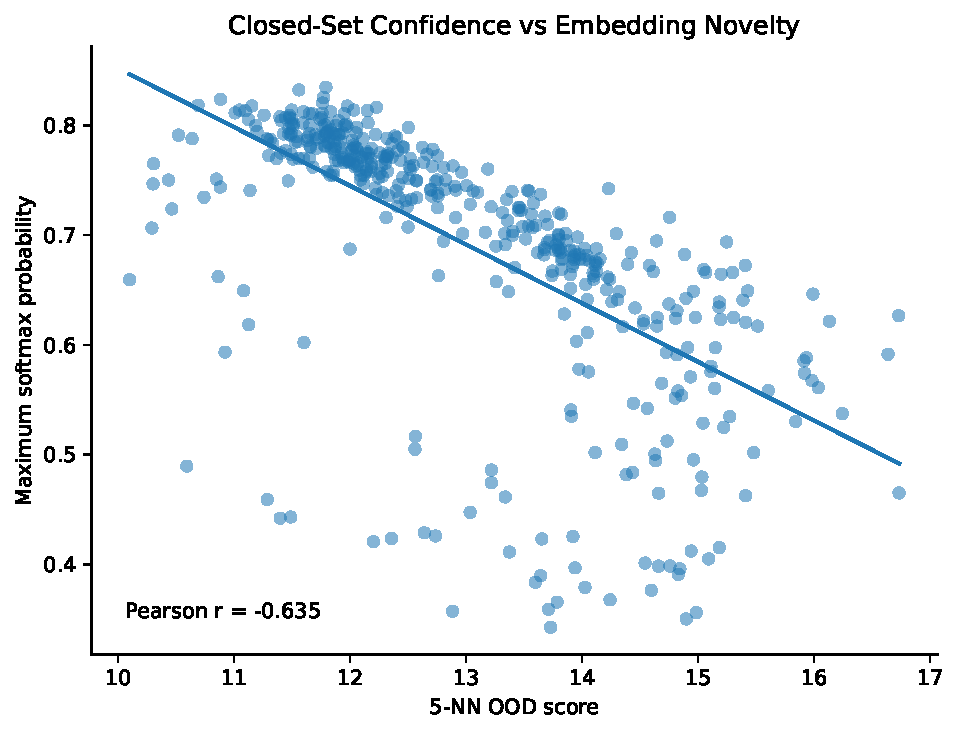
\includegraphics[
        width=0.72\linewidth
    ]{fig04_softmax_vs_ood.pdf}
    \caption{
        Maximum closed-set softmax probability versus
        5-NN geometric novelty for the 450 natural-OOD
        videos.
    }
    \label{fig:softmax}
\end{figure}


\subsection{Landmark coverage}

Landmark detection coverage varies substantially across the
expanded natural-OOD set. Mean detection rate is 0.8091,
median detection rate is 0.9851, and the observed range is
0.1955--1.0000.

Coverage and 5-NN novelty are negatively correlated,

\[
r=-0.5842.
\]

This association is an important potential confound.
The experiment therefore does not establish that embedding
distance responds exclusively to lexical novelty; part of the
distance variation may reflect landmark quality or other
dataset differences.

\begin{figure}[t]
    \centering
    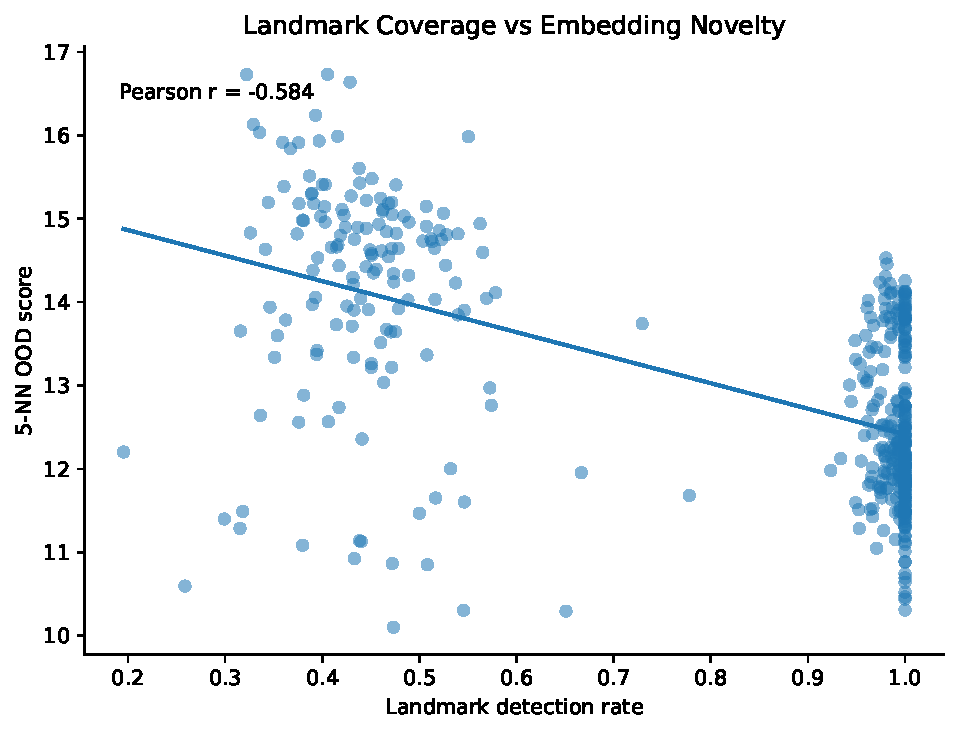
\includegraphics[
        width=0.72\linewidth
    ]{fig05_coverage_vs_ood.pdf}
    \caption{
        Landmark detection coverage versus 5-NN embedding
        novelty on the expanded natural-OOD set.
    }
    \label{fig:coverage}
\end{figure}


\section{Discussion}

The experiments reveal two distinct behaviours of the same
model. At the classifier output, unseen vocabulary is forced
into the four known categories. At the representation level,
however, the same inputs occupy regions that are substantially
farther from the training embedding bank than held-out
known-class inputs.

This distinction matters because softmax confidence answers
a conditional closed-set question: assuming the input must
belong to one of the supported classes, which class receives
the largest probability? It does not directly answer whether
that assumption is valid. Embedding distance provides a
separate signal addressing that second question.

The 94\% collapse of unseen vocabulary to \emph{my} is also
not merely a low-confidence ambiguity phenomenon. The
natural-OOD set has mean maximum softmax probability 0.6916,
and some unseen signs receive probabilities above 0.8.
A production interface displaying these predictions without
an explicit vocabulary-membership check could therefore
present unsupported classifications with apparently meaningful
confidence.

The geometric results suggest that useful open-set structure
can exist even when the original model was trained for
closed-set classification. This is attractive in a
low-resource setting because it permits an open-set layer to
be investigated without immediately retraining the underlying
network.

Nevertheless, the observed perfect ranking metrics should
not be overinterpreted. AUROC and AUPR of 1.0 describe the
finite datasets evaluated here. They do not imply that future
unknown signs, new recording environments, new signers, or
adversarially selected inputs will always be separated from
known classes.


\section{Limitations}

Several limitations constrain the conclusions of this study.

First, the known classifier vocabulary contains only four
glosses. This makes the baseline particularly narrow and may
increase the geometric separation between known and unseen
vocabulary. Open-set behaviour should be re-evaluated as the
known vocabulary grows.

Second, the natural-OOD videos originate from an external
dataset and may differ from the known-class data in ways
other than lexical identity. Differences in signer population,
camera characteristics, framing, motion, recording conditions,
or landmark quality could contribute to embedding separation.

Third, landmark coverage is correlated with the OOD score.
Although natural-OOD separation remains large in this
experiment, future work should explicitly disentangle lexical
novelty from extraction quality.

Fourth, the current threshold is based on empirical held-out
ID quantiles. A deployment threshold should be selected using
a dedicated calibration protocol and independently evaluated
on data not involved in threshold choice.

Finally, the checkpoint preprocessing was reconstructed for
compatibility. Although the resulting pipeline has been
audited experimentally, it is not claimed to reproduce
unpublished original training code exactly.


\section{Conclusion}

This work examines open-set failure in a four-class Kenyan
Sign Language Transformer baseline. The classifier is shown
to assign natural unseen-vocabulary KSL videos to known
classes with substantial confidence, with 94.0\% of 450
external test videos collapsing to the class \emph{my}.

The model's 256-dimensional representation tells a different
story. Mean nearest-neighbour distance to a training embedding
bank strongly separates the evaluated held-out known-class
samples from the 30-gloss natural unseen-vocabulary set.
For $k=5$, the maximum observed held-out ID score is 7.4174
and the minimum natural-OOD score is 10.1010. Across all
tested neighbourhood sizes, the present dataset yields
AUROC and AUPR of 1.0000.

The central implication is therefore not that open-set KSL
recognition is solved, but that closed-set probability and
vocabulary membership are materially different quantities.
For this baseline, explicitly modelling the latter through
representation geometry provides a substantially more
appropriate mechanism for rejecting the evaluated unseen
signs.

\end{document}